\subsection{Infrastruttura di supporto}

L'avvio dell'infrastruttura di monitoraggio è gestito dallo script 
\texttt{StartMetrics.sh}, che inizializza come container Docker tutti 
i servizi necessari al funzionamento del sistema.  
\begin{figure}[H]
    \centering
    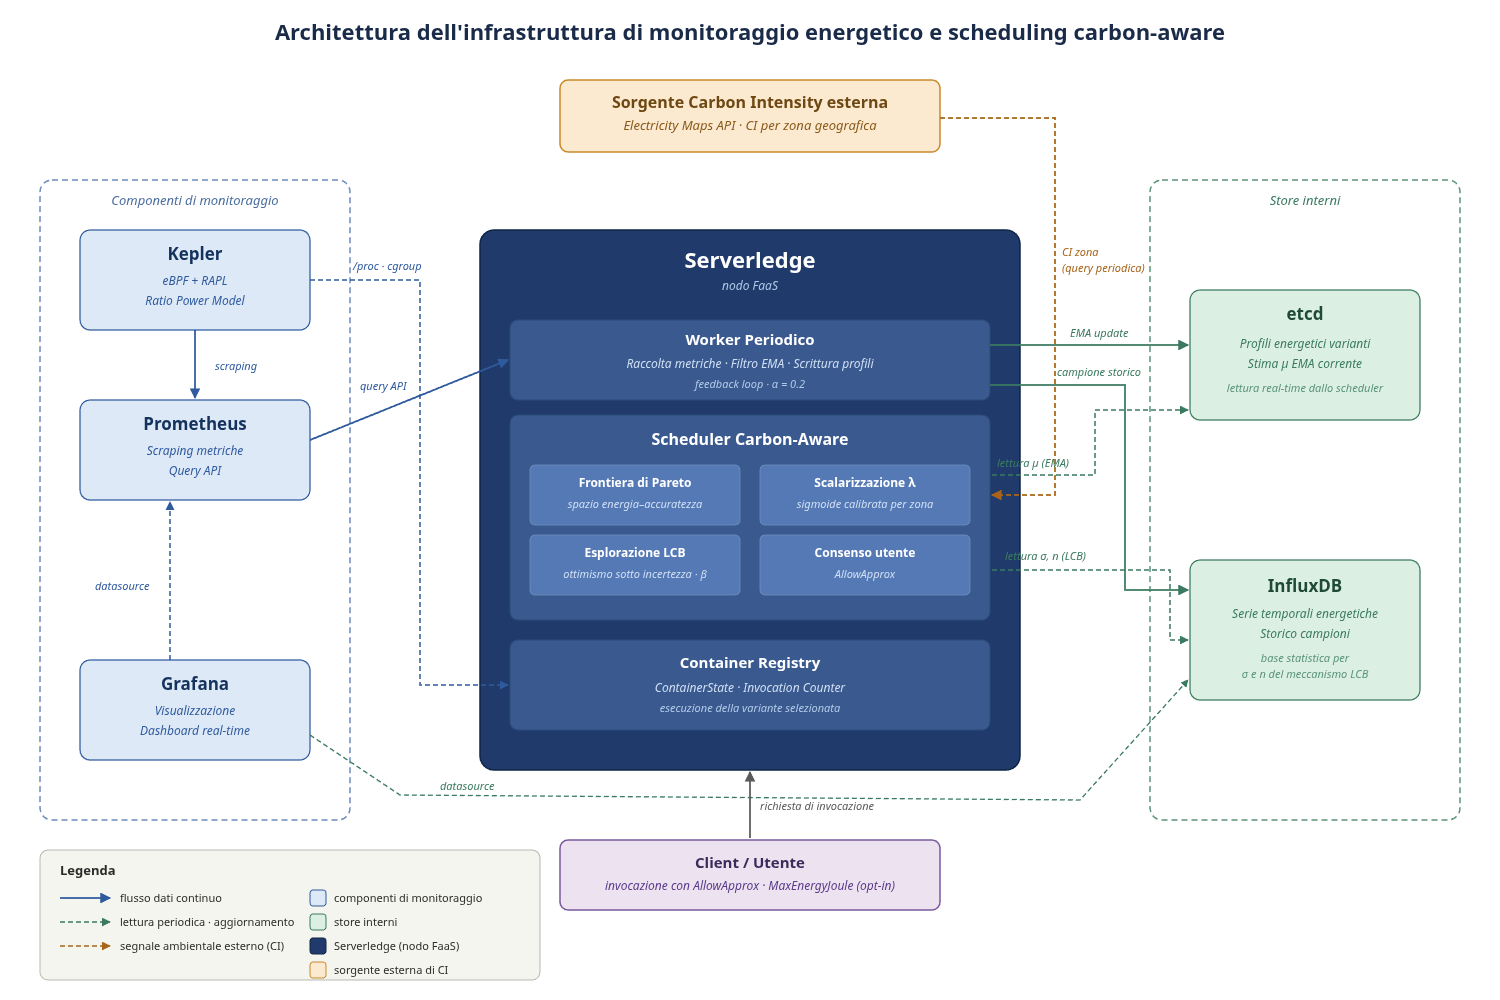
\includegraphics[width=0.85\textwidth]{figures/infrastracture-diagram.png}
    \caption{Architettura dell'infrastruttura di monitoraggio energetico e scheduling
carbon-aware. I componenti di monitoraggio esterni (Kepler, Prometheus, Grafana)
sono separati dagli store interni (etcd, InfluxDB), con Serverledge al centro
che interagisce con entrambi i livelli. Lo scheduler carbon-aware integra la
logica di selezione della variante — basata su frontiera di Pareto, scalarizzazione
tramite $\lambda$, esplorazione LCB e consenso utente — e riceve il segnale di
carbon intensity tramite query periodica a una sorgente esterna.}
    \label{fig:infra-arch}
\end{figure}

I componenti avviati,  come mostrato anche in Figura~\ref{fig:infra-arch}, sono i seguenti:

\begin{itemize}
    \item \textbf{Kepler}: eseguito in modalità privilegiata con accesso
 a \texttt{/sys}, \texttt{/proc} e al socket Docker dell'host, 
    condizioni necessarie per la lettura dei contatori RAPL e 
    l'associazione dei consumi ai container tramite cgroup.
    
    \item \textbf{Prometheus}: configurato per effettuare lo scraping 
    periodico delle metriche esposte da Kepler, rendendole disponibili 
    tramite API di interrogazione.
    
    \item \textbf{InfluxDB}: database a serie temporali utilizzato per 
    l'archiviazione storica dei campioni energetici prodotti dal 
    sistema ad ogni ciclo di raccolta.
    
    \item \textbf{etcd}: store distribuito chiave-valore che funge da 
    registro delle funzioni e delle relative varianti, inclusi i profili 
    energetici aggiornati dinamicamente a runtime.
    
    \item \textbf{Grafana}: strumento di visualizzazione utilizzato per 
    il monitoraggio in tempo reale dei consumi durante gli esperimenti.
\end{itemize}

Una volta avviata, l'infrastruttura opera in modo autonomo: Kepler 
rileva i container Docker presenti sull'host e ne aggiorna le metriche 
energetiche ad ogni ciclo di campionamento; Prometheus le raccoglie e 
le rende interrogabili; il sistema interno di Serverledge, descritto nelle sezioni successive,
le legge periodicamente --- limitatamente ai container attivi da esso gestiti --- per aggiornare i profili energetici 
delle varianti di funzione. Il segnale di carbon intensity, necessario allo scheduler 
per la selezione carbon-aware della variante, non è parte di questa infrastruttura: 
viene acquisito dallo scheduler a runtime tramite query periodica a una 
sorgente esterna, come descritto nella Sezione~\ref{cap:scheduler}.